
\begin{frame}
 \frametitle{Normal diffusion}
 \begin{itemize}
  \item Process of net movement due to a difference in concentration.
  \item Formulated in 1855 by Adolf Fick in the modern way.
  \item Widely used across many diciplines like social studies, economics and biology.
 \end{itemize}

 \begin{equation*}
  \frac{\d C}{\d t} = D\nabla^2C
 \end{equation*}
\begin{figure}[H]
 \centering
 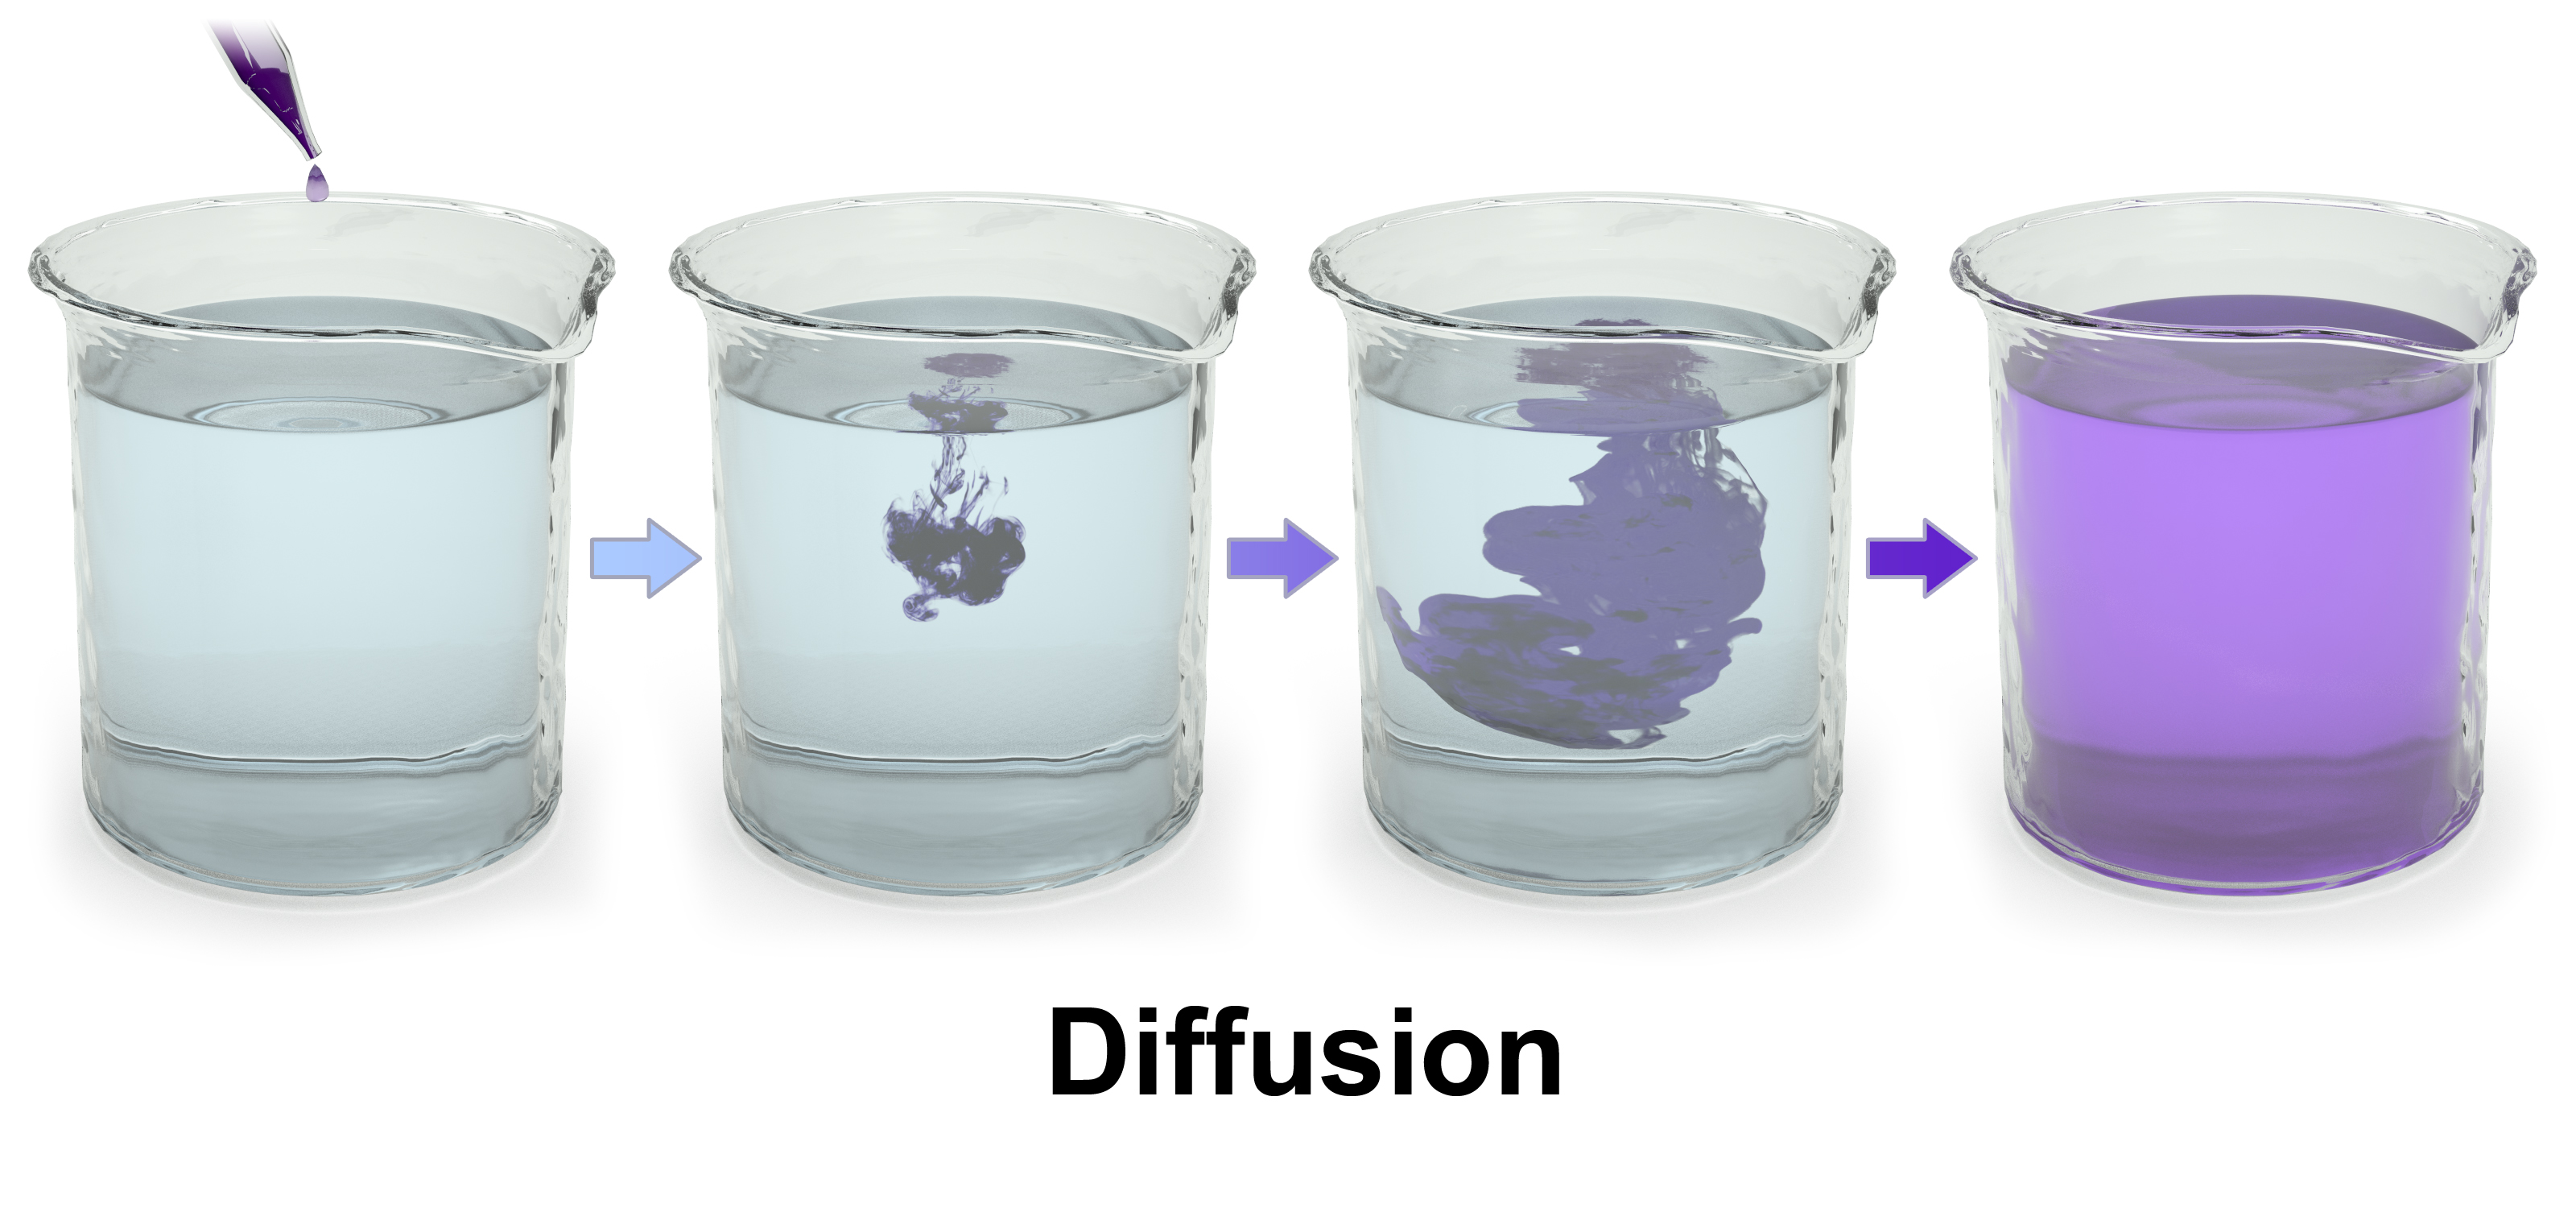
\includegraphics[width=\textwidth]{figures/Diffusion.png}
\end{figure}

\end{frame}



\begin{frame}
 \frametitle{Random walks}
 \begin{columns}
  \column{0.48\textwidth}
  \begin{itemize}
   \item Also widely used in many diciplines.
   \item ``Endless'' possibilities for added complexity.
   \item Conceptually not that difficult.
   \item Recreates diffusion
  \end{itemize}
\column{0.48\textwidth}
\begin{figure}[H]
\centering
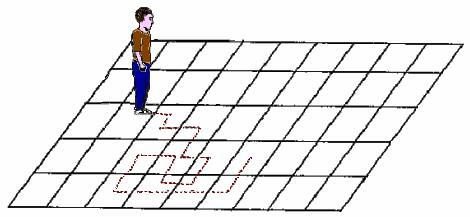
\includegraphics[width=\textwidth]{figures/RW.jpg}
 \end{figure}

 \end{columns}
\end{frame}